%%==================================================
%% chapter4.tex for BIT Master Thesis
%% version: 0.1
%% last update: Nov 8th, 2017
%%==================================================
\chapter{离散时间半参数自适应控制}\label{chap:4}
自适应控制中的的辨识是为了控制问题,上一章设计了二维情形下的信息浓缩估计算法去辨识线性部分的未知参数。本章将在第三章的基础上设计非参数部分的估计算法,主要借助于一种机器学习算法,然后根据两部分的估计结果去设计自适应控制律在去解决随动控制问题。
\section{问题描述}\label{sect:4.1}
再次考虑第二章给出的半参数模型
\begin{equation}%
\label{eq:4.semi-u}
y_{k+1} = \bm{\theta}^{T}\bm{\phi_{k}}+u_{k}+f(\bm{\psi_{k}})+\omega_{k+1}
\end{equation}
其中,$\bm{\theta}$是未知参数向量,$f(\cdot)$是未知函数。同理,令
\begin{equation}
z_{k} = f(\psi_{k}) + \omega_{k+1}
\end{equation}

针对系统\eqref{eq:4.semi-u},自适应估计与控制问题的一般表述是:给定关于$\bm{\theta}$,$f(\cdot)$和$\omega_{k+1}$的先验信息,如何根据实时产生的一系列输入输出数据$\{y_{k},u_{k};k=1,2,\ldots\}$,去估计未知参数$\bm{\theta}$和$z_{k}$?然后根据$\bm{\theta}$和$z_{k}$的估计(预测)值去设计合适的自适应控制输入$u_{k}$使得$k+1$时刻的输出$y_{k+1}$能跟踪上期望的输出$y_{k+1}^{*}$。

第三章已经给出了$\bm{\theta}$的估计算法,因此剩下的部分可以分为两个核心问题,一方面是设计$f(\cdot)$的估计算法,另一方面是设计控制输入$u_{k}$的表达式。假设第二章设计出的未知参数的估计值为$\hat{\bm{\theta}}_{k}$,下面需要设计出$\breve{z}_{k}$的表达式。因此,根据必然等价原理,设计出的控制输入的一般表达式为:
\begin{equation}\label{eq:4.uk}
u_{k}^{*}=y_{k+1}^{*}-\bm{\phi_{k}}^{T}\cdot\hat{\bm{\theta}}_{k}-\breve{z}_{k}
\end{equation}

\section{超限学习机}\label{sect:4.2}

人工智能的发展一直推动着神经网络的研究,特别是2012年之后,深度学习(Deep Learning, DL)在图像分类、语音识别、自然语言处理等应用领域中获得了巨大成功\upcite{ZhengChenZhang2014}。目前大部分的深度学习算法大部分是基于神经网络建立。对于深度学习来说,隐含层的数量级为十几层到几百层不等,甚至上千层。深层网络结构和特征学习思想是深度学习的两大主要特点。与深度学习相比,超限学习机在不丢失精度的条件下具有快速的优势,比较见图\ref{fig:elm-dl}所示。

\begin{figure}
 \centering
 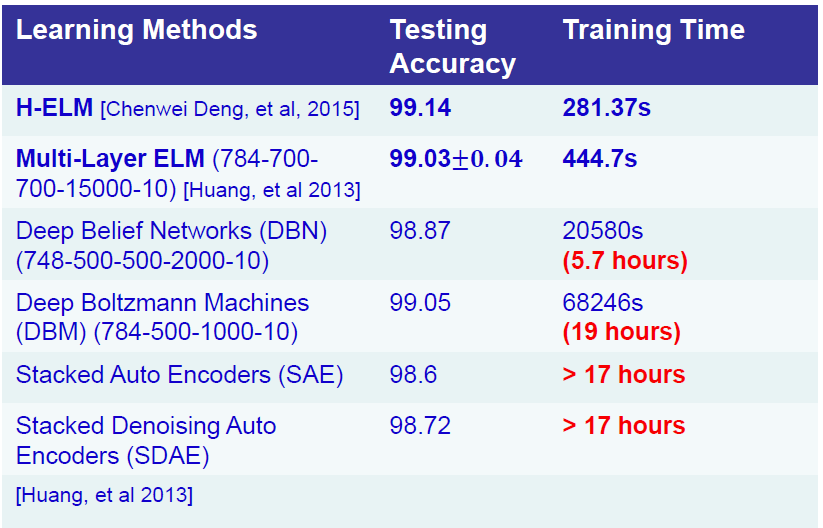
\includegraphics[width=0.7\textwidth]{figures/elm-dl}
 \caption{超限学习机与常见深度学习性能比较}\label{fig:elm-dl}
\end{figure}
